%% Report template.
%% Author: Kim Hammar
\documentclass[a4paper, 11pt]{article}
\usepackage{graphicx}
%\usepackage[T1]{fontenc}
\usepackage[utf8]{inputenc} 
%\usepackage[swedish]{babel}
\usepackage{graphicx}
\usepackage{cite}
\usepackage{natbib}
\usepackage{url}
\usepackage{float}
\usepackage{vhistory}
\usepackage{lastpage}
\usepackage{fancyhdr}
\usepackage{lettrine}
\graphicspath{ {./images/} }
\usepackage{hyperref}
\hypersetup{
    colorlinks,
    citecolor=black,
    filecolor=black,
    linkcolor=black,
    urlcolor=black
}
\pagestyle{fancy}
\fancypagestyle{firststyle}
{
  \lhead{}
  \chead{}
  \rhead{\textbf{Course project} ID2212}
   \fancyfoot[C]{\footnotesize Page \thepage\ of \pageref{LastPage} }
}
  \lhead{}
  \chead{}
  \rhead{\leftmark}
  \fancyfoot[C]{\footnotesize Page \thepage\ of \pageref{LastPage} }

\title{Course project}
\author{Kim Hammar}
\date{7 dec 2015}
\begin{document}
\maketitle
\thispagestyle{firststyle}
\begin{versionhistory}
\vhEntry{0.1}{07.12.15}{KH}{First draft}
\vhEntry{0.2}{13.12.15}{KH}{Error correction}
\end{versionhistory}
\newpage
\tableofcontents
\newpage

%\begin{figure}[H]
%\includegraphics[scale=0.5]{klass.png}
%\caption{Konceptuell modell över systemet}
%\end{figure}
\section{Abstract}
Course project in a course on Network programming in Java \citep{kth_1}, carried out at Royal Institute of Technology, Stockholm.
\newpage
\section{Task specification}
\textit{You are ``hired'' by JEM inc (Java Enterprise Microsystems Inc.) to design and develop the distributed application software (clients and servers) for the NOG (Nordic Olympic Games) event.} \\ \\
The NOG information system should allow storing, retrieving and updating personal information about NOG participants. The system should also be able to provide statistical information about participants. The system is to be developed in two version(1) a single-user version; (2) a multi-user version. \\ 
You should also develop a NOG virtual meeting place. The NOG virtual meeting place is Internet based software which offers remotely located users to communicate and share information represented as textual, image or audio files. 
\subsection{Sub-assignment 1. A Single-User Information System for NOG}
Develop a distributed application in Java that allows storing, retrieving and updating information about participants of NOG. The application should concist of a client with a user interface and a server. In this assignment we assume a \textbf{single user} semantics for the application, i.e It's not required to support coherency of multiple copies of participant records which may be cached by multiple client at the same time.
\subsection{Sub-assignment 2. A Multi-User Information System for NOG}
Develop a multi-user application, similar to the solution developed in sub-assignment 1. In this version a multi-user semantic is required. Many users can fetch the participants-data at the same time and when one user updates his local-cache of the data, the change need to be replicated among all clients connected in order to prevent them from using stale data.
\subsection{Sub-assignment 3. Chat Rooms for NOG}
Develop a distributed ``building of chat rooms''.

\newpage
\section{Platform}
The platform used for the devlopment-process, benchmarks and tests is a computer running Xubuntu 14.04 LTS, CPU: Intel(R) Core(TM) i7-4790 CPU @ 3.60GHz \\ \\
Java version: 1.7.0\_79  (OpenJDK version 7 update 79).
\section{Software and technologies used}
\begin{itemize}
\item Java Remote Method Invocation (java.rmi package)
\item Java Persistence API (javax.persistence package)
\item JDBC (java.sql package)
\item Java Swing (javax.swing package)
\item Java Socket (java.net package)
\item PostgreSQL 9.3.9
\item Apache JMeter
\end{itemize}
\newpage
\section{The application}
\subsection{Sub-assignment 1. A Single-User Information System for NOG}
\subsubsection{Functionality}
Distributed java application that allows storing and updating information about participants in NOG. The server is using the HTTP protocol and only supports GET and PUT methods (PUT For storing and GET for fetching). The server is multithreaded but doesnt provide any multi-user semantics in the likes of keeping consistent data among clients (hence the minimized protocol of GET/PUT).
\\\\The client is a simple http-client atached with a GUI developed with Java Swing.
\subsubsection{Protocols used}
\begin{itemize}
\item HTTP 
  \begin{itemize}
  \item PUT/GET methods.
  \end{itemize}
\end{itemize}
\subsubsection{GUI}
\begin{figure}[H]
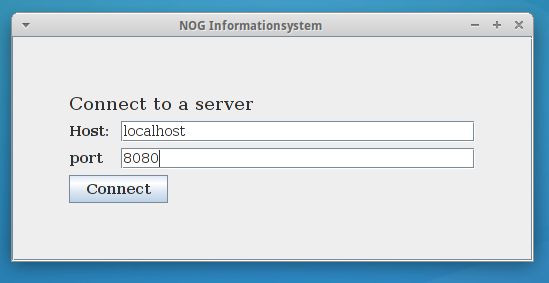
\includegraphics[scale=0.60]{assignment1_1.png}
\caption{Screenshot of the startframe of the application}
\end{figure}
\begin{figure}[H]
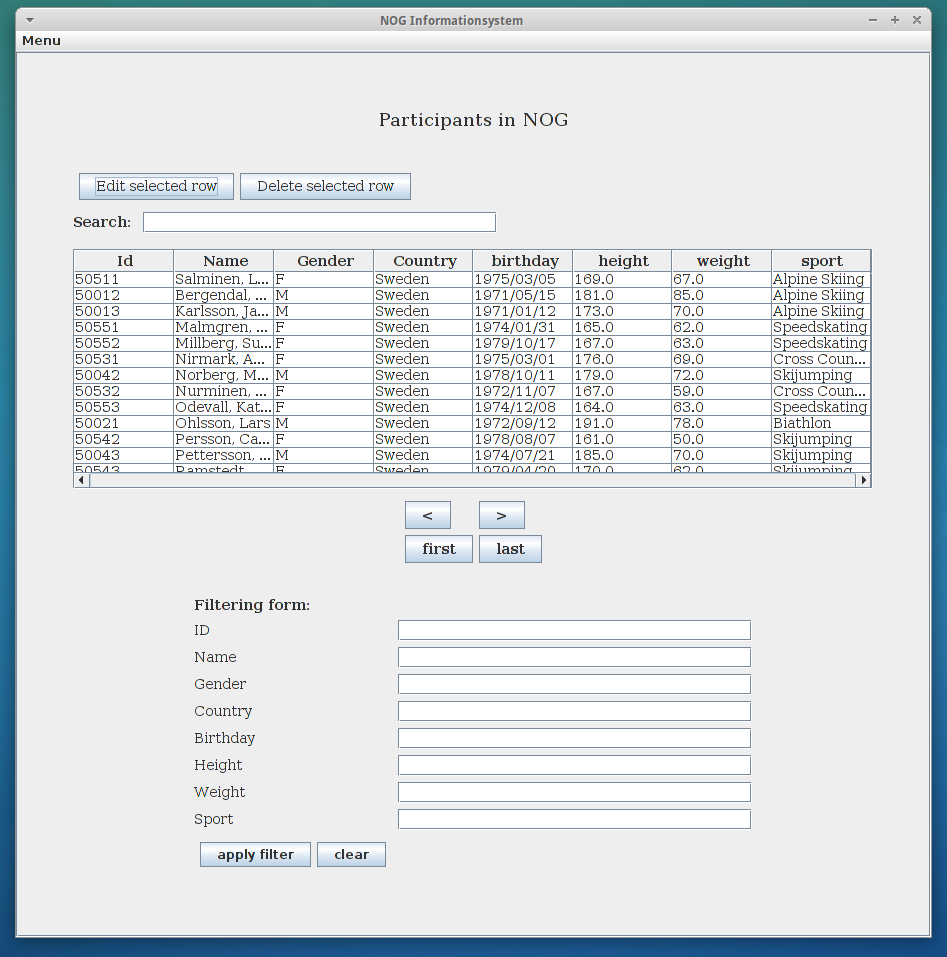
\includegraphics[scale=0.40]{assignment1_2.png}
\caption{Screenshot of the mainPanel of the application}
\end{figure}
\begin{figure}[H]
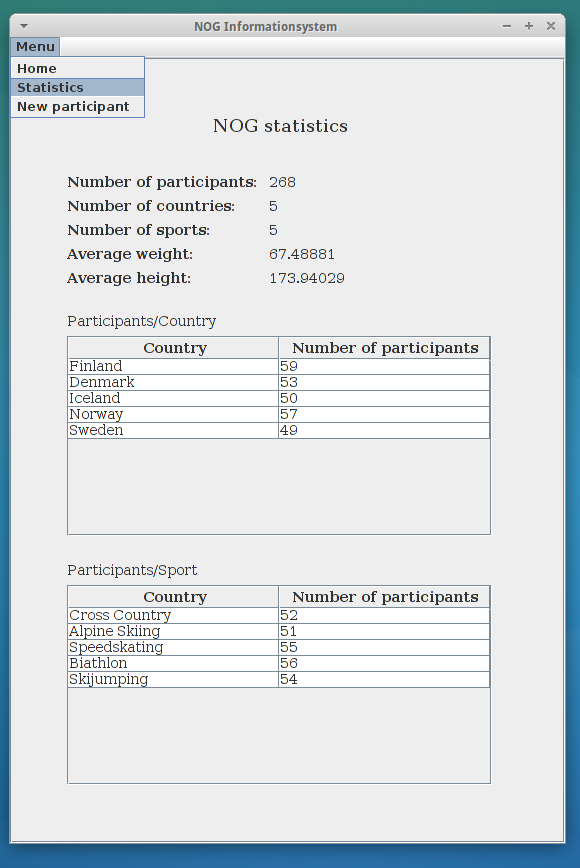
\includegraphics[scale=0.60]{assignment1_3.png}
\caption{Screenshot of the statisticsPanel of the application}
\end{figure}
\begin{figure}[H]
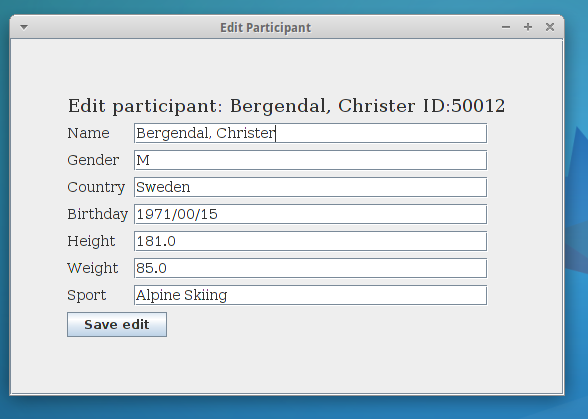
\includegraphics[scale=0.60]{assignment1_5.png}
\caption{Screenshot of the EditPanel of the application}
\end{figure}
\subsubsection{Architecture}
\begin{figure}[H]
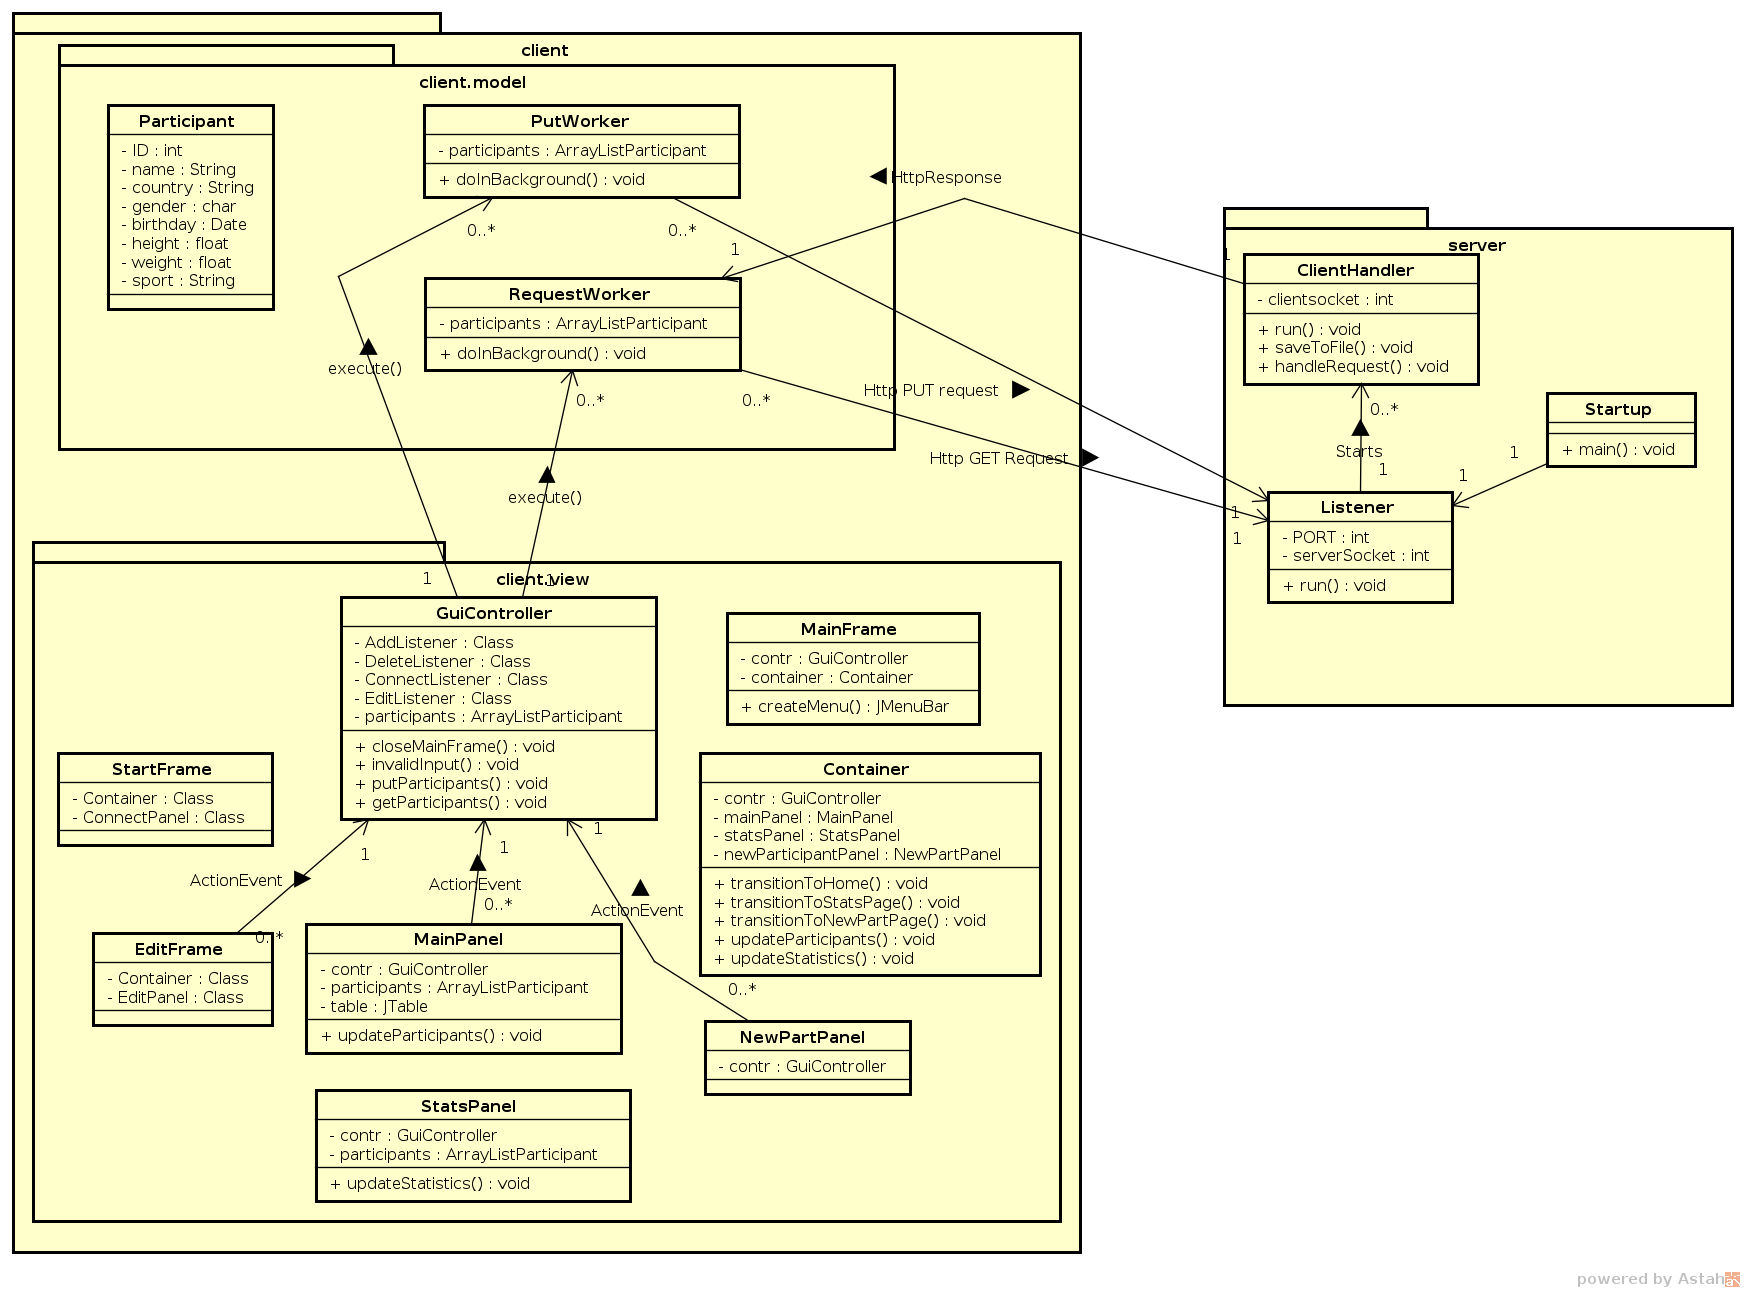
\includegraphics[scale=0.35]{assignment1_architecture.png}
\caption{Class diagram over the application architecture.}
\end{figure}
\subsubsection{Load-testing}
These tests have been done on my local machine so It is'nt a real proof of how the application would hold under huge loads in production but we can still see some interesting results.
My main purpose with this load test was to see how well the multi-threaded semantics is working in reality. Since the test-environment is on a machine with 7 cores, we can expect that the througput would be higher when there is multiple clients sending requests concurrently. \\
\textbf{Without latency simulation}
%%Table with borders 
\begin{table}[H]
\centering
\label{Load-test for http-server}
\begin{tabular}{|l|l|l|r|}
\hline
\textbf{No. threads}  & \textbf{No. requests}  & \textbf{Throughput/sec} & \textbf{(KB/sec)} \\ \hline
1Thread & 100 & 990.099 & 17579.091 \\ \hline
2Threads & 100 & 1470.588 & 26110.122 \\ \hline
4Threads & 100 & 1886.792 & 33499.779 \\ \hline
10Threads & 100 & 2631.579 & 46723.376 \\ \hline
TOTAL & 400 & 1486.989 & 26401.313 \\ \hline
\end{tabular}
\caption{Load-test for http-server}
\end{table}
\begin{figure}[H]
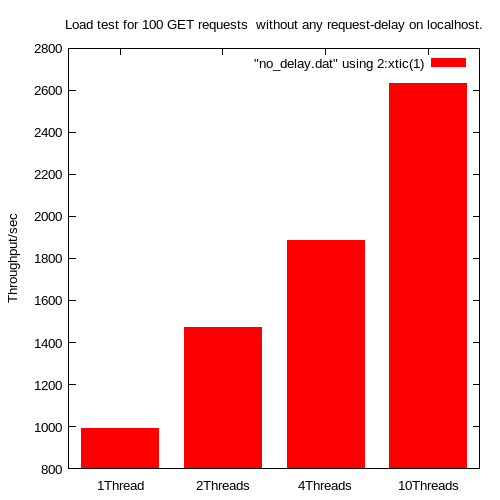
\includegraphics[scale=0.7]{no_delay.png}
\caption{Throughput/sec for different number of threads}
\end{figure}
The result show that 10 threads gave more than doubled the througput compared to 1 thread. But it was'nt the result I expected. \\
I expected a linear growth in throughput with respect to number of threads until we reach $\approx 7$ threads (which is the maximum number of threads that can run in parallell on the test-machine) where the througput would stabilize around some value. \\ \\ 
\textbf{With latency simulation} \\ 
Since the server was running on my local machine it barely was'nt any latency between the requests at all, I figured that was the reason the tests did'nt match my expectations.
To simulate network-latency that might occur outside of the test-environment I added a 200 millisecond delay at the server while handling the requests and re-did the tests to see what  effect it gave.
%%Table with borders 
\begin{table}[H]
\centering
\label{Load-test for http-server with latency simulation}
\begin{tabular}{|l|l|l|r|}
\hline
\textbf{No. threads}  & \textbf{No. requests}  & \textbf{Throughput/sec} & \textbf{(KB/sec)} \\ \hline
1Thread & 100 & 4.946 & 87.817 \\ \hline
2Threads & 100 & 9.870 & 175.253 \\ \hline
4Threads & 100 & 19.685 & 349.505 \\ \hline
10Threads & 100 & 49.189 & 873.334 \\ \hline
TOTAL & 400 & 10.672 & 189.486 \\ \hline
\end{tabular}
\caption{Load-test for http-server with latency simulation}
\end{table}
\begin{figure}[H]
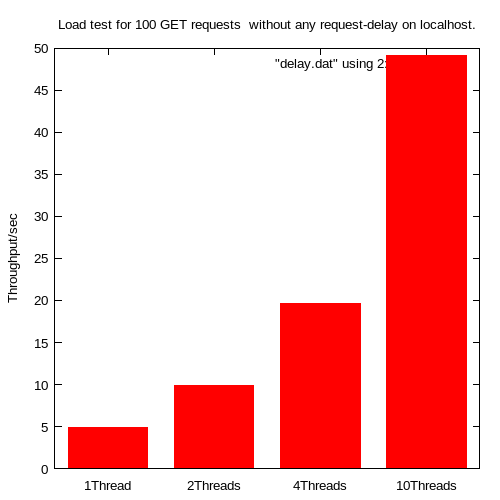
\includegraphics[scale=0.7]{delay.png}
\caption{Throughput/sec for different number of threads}
\end{figure}
As can be seen from the benchmark-results with the latency-simulation, the througput is much lower, obviously.

What's interesting here is the througput gains we get by having multiple threads issuing the requests in parallell, we can see that 10 threads issuing GET-requests in semi-parallell give $\approx 10$ times higher througput/sec than 1 thread.
\subsection{Sub-assignment 2. A Multi-User Information System for NOG}
\subsubsection{Functionality}
A multi-user distributed application that allows storing, fetching and updating (delete, edit, add) participants data. The server is developed with Java RMI and the persistence layer is developed with JPA (Java Persistence API). The underlying database is PostgreSQL. \\ \\
The server is multithreaded (with java rmi) and provides functionality to let many user at a time update and have local copies of the data where every update will be replicated among every other user that is connected.
\\\\ The client is a simple Java RMI client with a Java Swing GUI.
\subsubsection{Protocols used}
Custom developed protocol for remote method calls between server and client. \\
\textbf{Server-interface:}
\begin{itemize}
\item getParticipants
\item putParticipants
\item addParticipant
\item deleteParticipant
\item editParticipant
\end{itemize} 
\textbf{Client-interface:}
\begin{itemize}
\item updateParticipants
\end{itemize}
\subsubsection{GUI}
Same GUI as for sub-assigment 1.
\subsubsection{Architecture}
\begin{figure}[H]
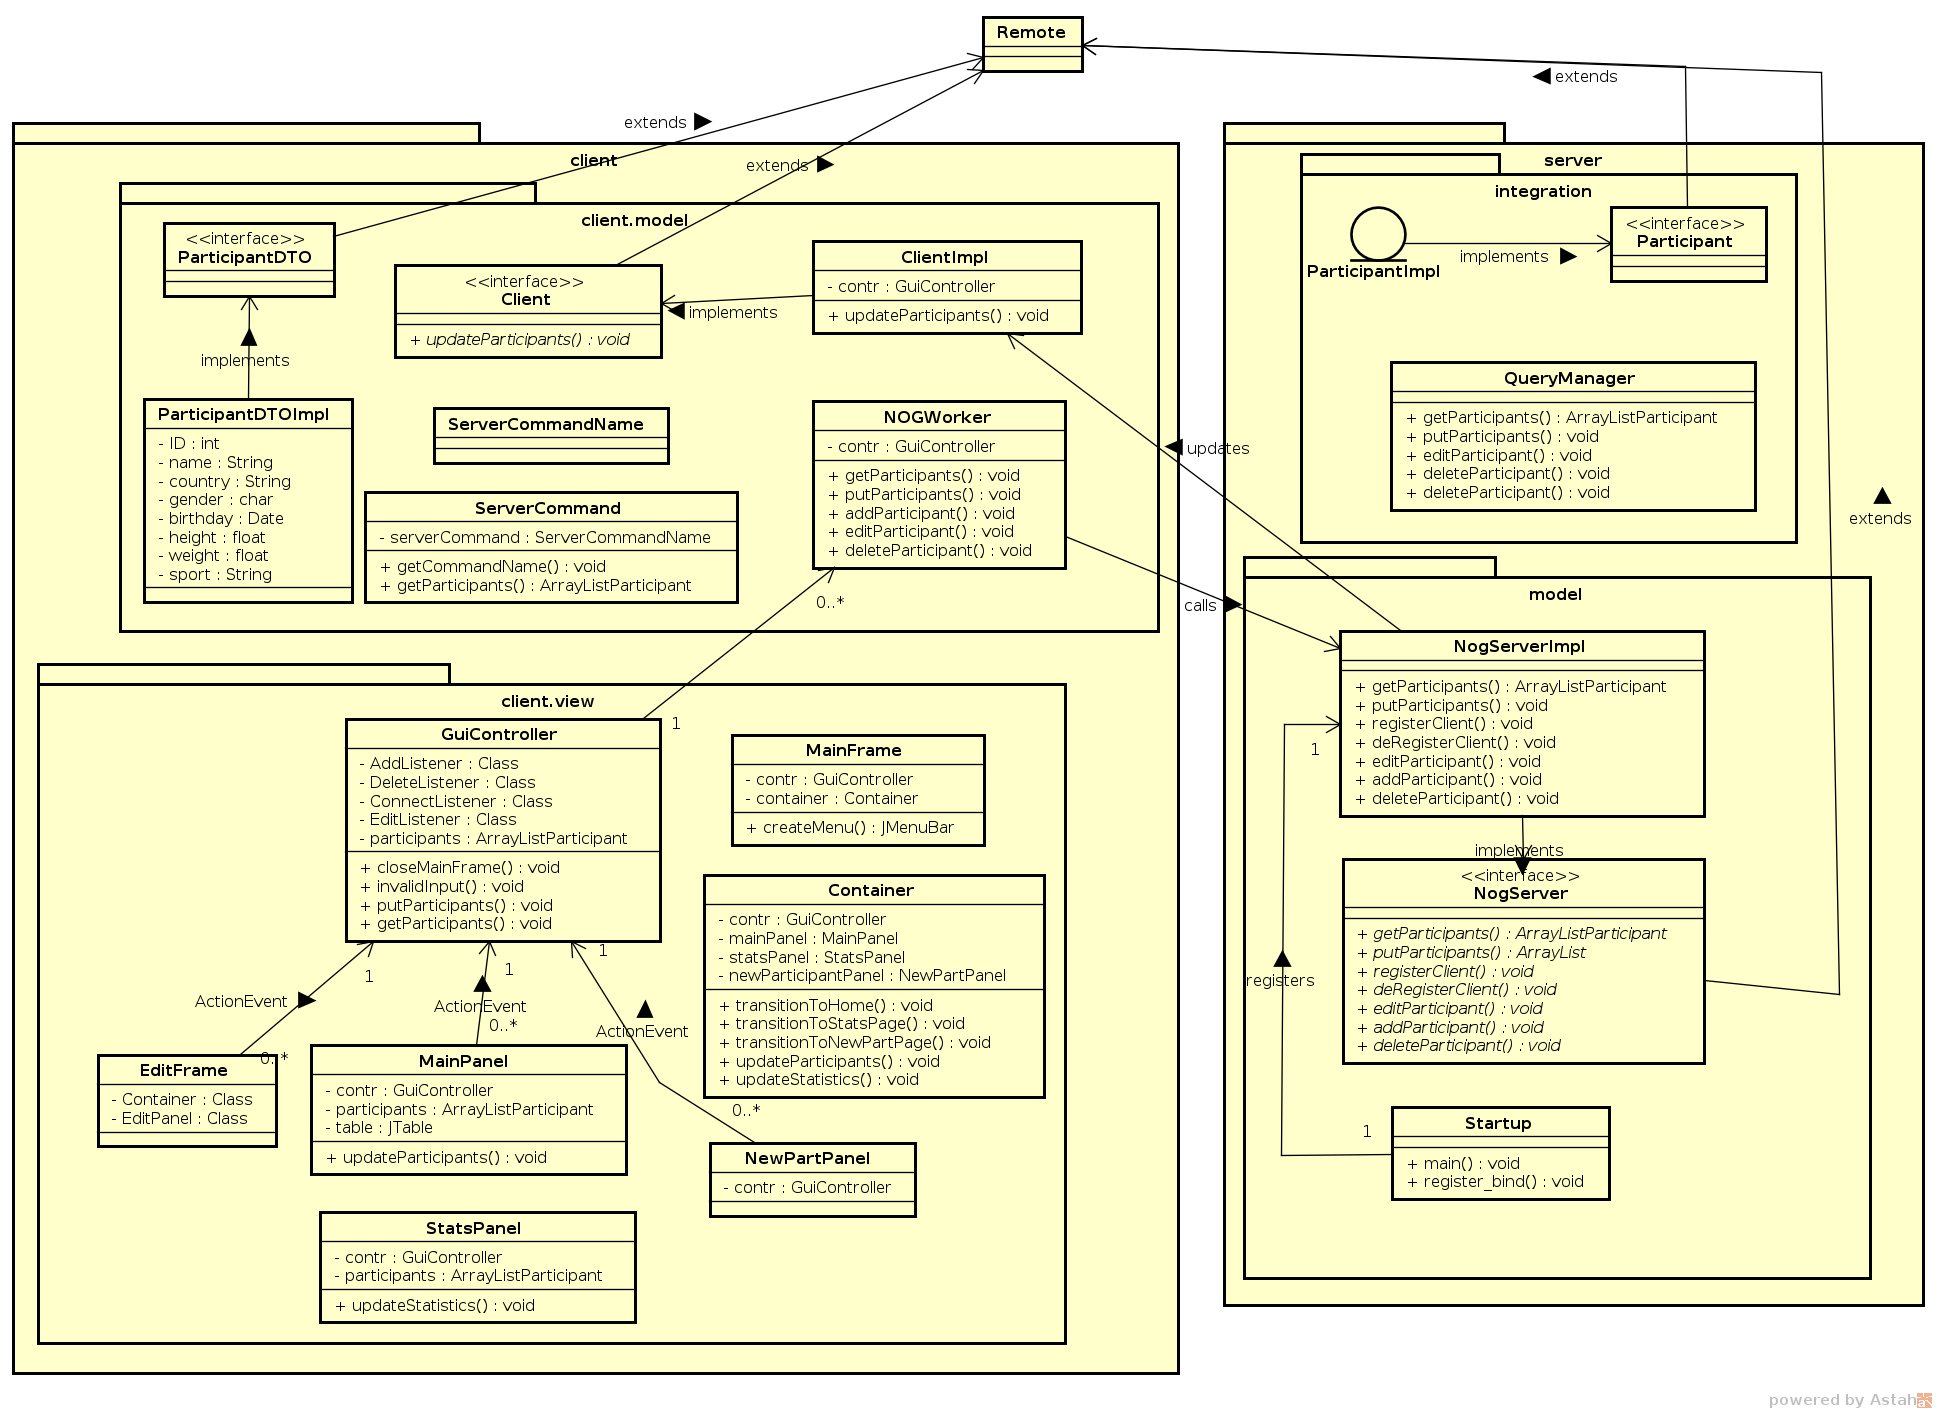
\includegraphics[scale=0.30]{assignment2_architecture.png}
\caption{Class diagram over the application architecture.}
\end{figure}
\subsubsection{Load-testing}
The loadtesting done for this assigment is of another nature than the tests done for sub-assignment 1. Here i have created a custom LoadTesting class for issuing remote method-calls to the RMI-server all method-calls is done single-threaded. An important note here is that all of these functions contains database interaction, so besides the Java RMI server these tests also depend on the database-layer which is in PostgreSQL. Just like for the load-testing done on the sub-assignment 1 http-server, number of calls done for each method is 100.\\
%%Table with borders 
\begin{table}[H]
\centering
\label{Performance test for rmi-server}
\begin{tabular}{|l|l|r|}
\hline
\textbf{Method}  & \textbf{No. calls} & \textbf{Time (s)} \\ \hline
getParticipants	& 100 & 0.926 \\ \hline
addParticipant	& 100 & 0.293 \\ \hline
deleteParticipant & 100 & 0.110 \\ \hline
deleteParticipant & 100 & 0.211 \\ \hline
\end{tabular}
\caption{Performance-test for rmi-server}
\end{table}
\begin{figure}[H]
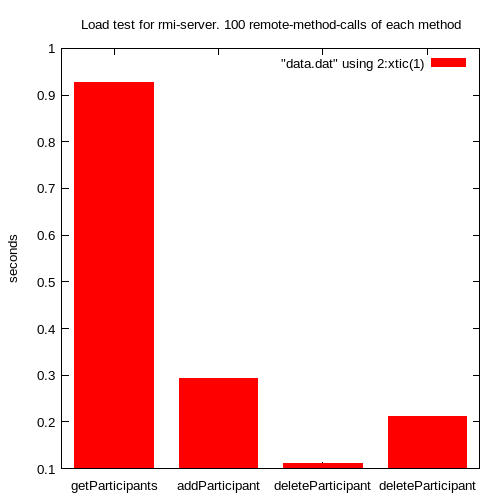
\includegraphics[scale=0.7]{rmiplot.png}
\caption{Benchmark results.}
\end{figure}
The result is not very suprising, \textit{getParticipant} is by far the method that takes the most  time and \textit{deleteParticipant} takes the least. \\

This was not a sophisticated load-test but we can still see that the rmi-server is alot slower than the http-server in sub-assignment 1, if we convert the data in the table above we can get that the rmi-server can handle 100 calls for getParticipants in $\approx 0.92$ seconds. In comparison with the load-test result from sub-assignment 1 (the single-threaded version) which could handle $\approx 990$ GET-requestst of the participants, the rmi-server is way slower. The fact that the rmi-server is slower than the http-server is not suprising since the http-server simply reads from a tsv file while the rmi-server goes through many more steps: conversion from relational data to object-data with the ORM, compile psql-commands down to sql etc. but I did'nt expect the differencies to be this big.
\subsection{Sub-assignment 3. Chat Rooms for NOG}
\subsubsection{Functionality}
Distributed chat application for NOG users.
The server is deveoped with java RMI and provides functionality for users to create/destroy/add chatrooms, to Direct-Message other users and to block users.
\\ \\The client is developed with java-rmi and is attached with a GUI developed with java Swing.
\subsubsection{Protocols used}
Custom developed protocol for remote method calls between server and client. \\
\textbf{Server-interface:}
\begin{itemize}
\item getClients
\item registerClient
\item deRegisterClient
\item getChatRooms
\item addChatRoom
\item sendMessage
\item joinChat
\item destroyChatRoom
\item leaveChatRoom
\item privateChatRoom
\end{itemize}
\textbf{Client-interface:}
\begin{itemize}
\item updateClients
\item updateChatRooms
\item updateChat
\item chatRoomDestroyed
\item BlockClient
\item unBlockClient
\item getBlockedList
\end{itemize}
\subsubsection{GUI}
\begin{figure}[H]
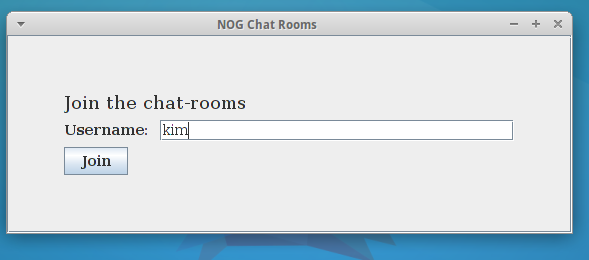
\includegraphics[scale=0.60]{assignment2_1.png}
\caption{Screenshot of the startframe of the application}
\end{figure}
\begin{figure}[H]
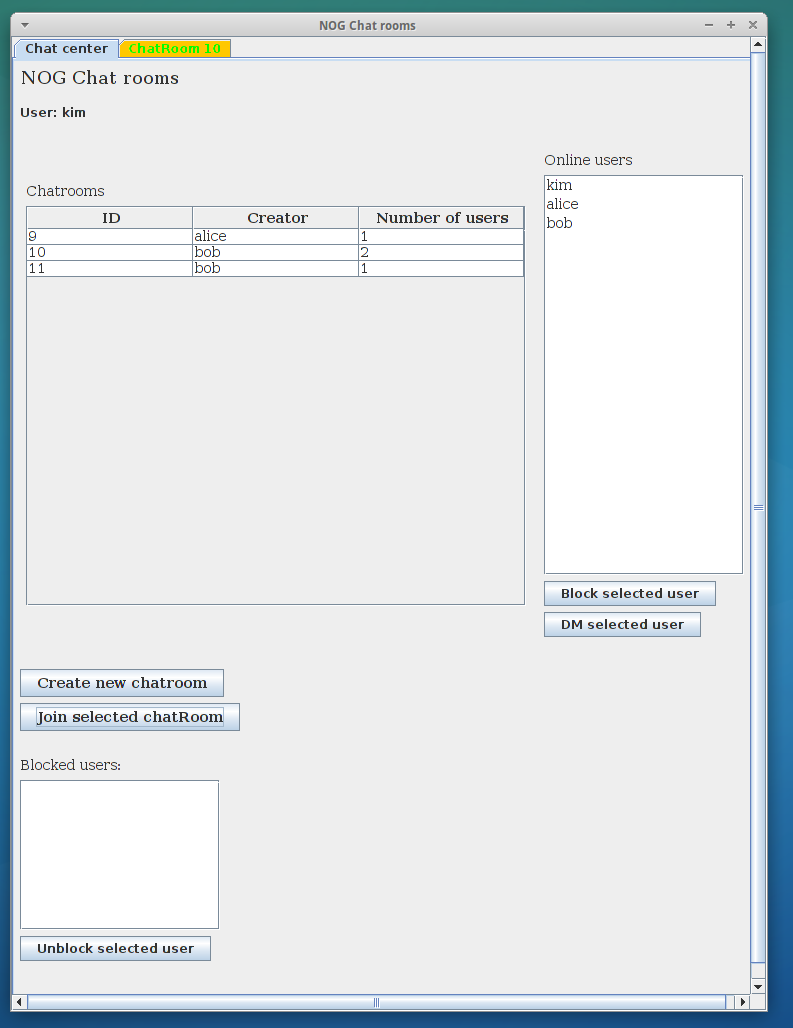
\includegraphics[scale=0.50]{assignment2_3.png}
\caption{Screenshot of the MainPanel of the application}
\end{figure}
\begin{figure}[H]
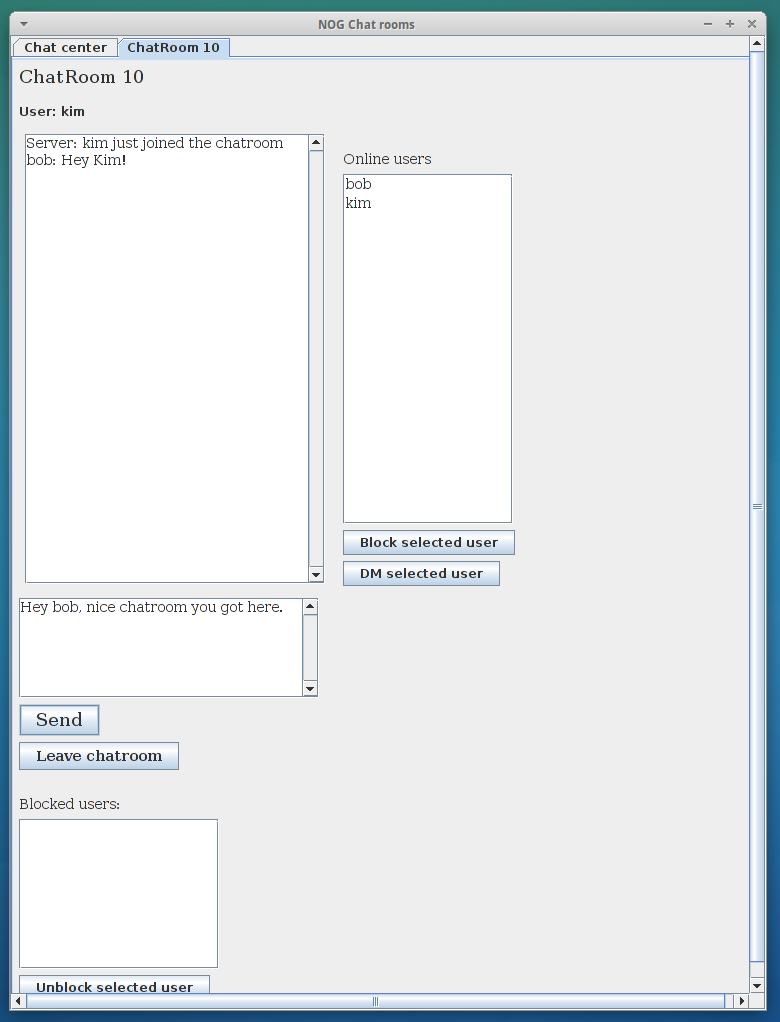
\includegraphics[scale=0.50]{assignment2_4.png}
\caption{Screenshot of the MainPanel of the application}
\end{figure}
\subsubsection{Architecture}
\begin{figure}[H]
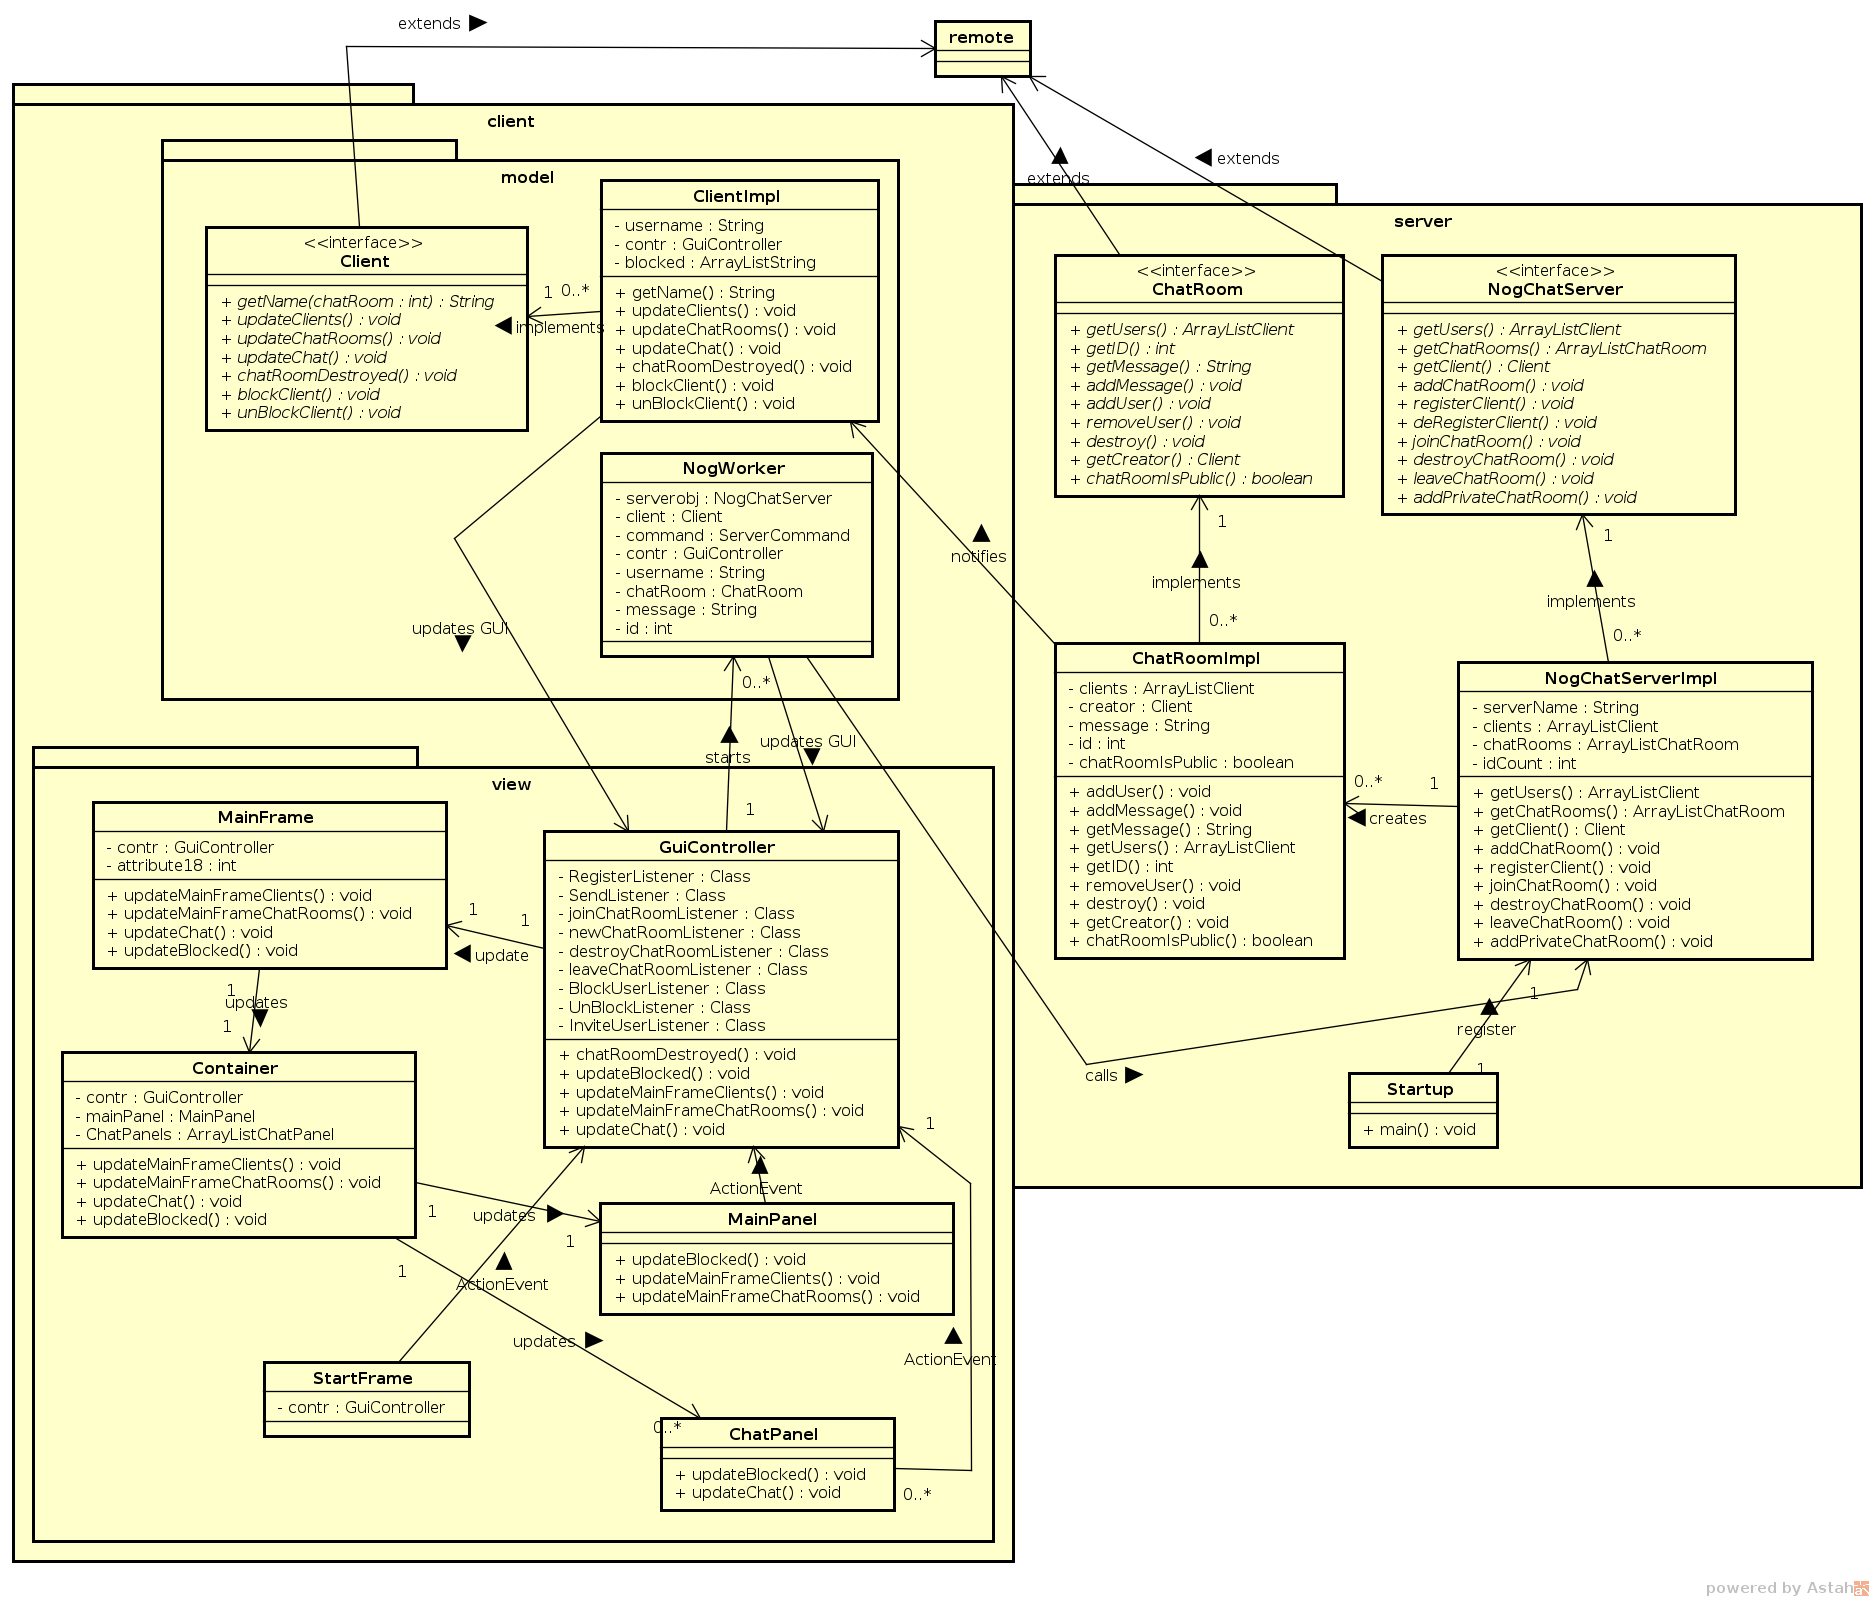
\includegraphics[scale=0.30]{assignment3_architecture.png}
\caption{Class diagram over the application architecture.}
\end{figure}
\section{Documentation}
\newpage
\nocite{*}
\bibliographystyle{plain}
\bibliography{references}
\end{document}


%%% Local Variables:
%%% mode: latex
%%% TeX-master: t
%%% End:

%\textbf // bold
%\textit // italic

%%Punktlista
%%
%%\begin{itemize}
%%  \item The first item
%%  \item The second item
%%  \item The third etc \ldots
%%\end{itemize}

%% Numrerad lista
%%
%%\begin{enumerate}
%%  \item The first item
%%  \item The second item
%%  \item The third etc \ldots
%%\end{enumerate}

%%table without borders:
%%\begin{table}[]
%%\centering
%%\label{my-label}
%%\begin{tabular}{llr}
%%Animal     & Description & Price (\$) \\ \hline
%%Gnat       & per gram    & 13.65      \\
%%           & each        & 0.01       \\
%%Gnu        & stuffed     & 92.50      \\
%%Emu        & stuffed     & 33.33      \\
%%Armadillo  & frozen      & 8.99       \\ \hline
%%\end{tabular}
%%\caption{My caption}
%%\end{table}

%%Table with borders
%% 
%%\begin{table}[]
%%\centering
%%\label{my-label}
%%\begin{tabular}{|l|l|r|}
%%\hline
%%\textbf{Animal}      & \textbf{Description}  & \textbf{Price} \textit{(\$)} \\ \hline
%%Gnat        & per gram     & 13.65      \\ \hline
%%            & each         & 0.01       \\ \hline
%%Gnu         & stuffed      & 92.50      \\ \hline
%%Emu         & stuffed      & 33.33      \\ \hline
%%Armadillo   & frozen       & 8.99       \\ \hline
%%\end{tabular}
%\caption{My caption}
%\end{table}


%%C-c C-c //Kompilerar det som behöver kompileras (latex eller bibtex elr whatever, emacs är smart!
%%C-c C-v //Visa pdf
%%C-c = //Visa innehållsförteckningen
%%C-c C-k //Kill the TeX subprocess (tex-kill-job). 
%%C-c C-f // Invoke TeX on the current file (tex-file).
%%C-c C-l // se output av senaste kommandot, error meddelande t.ex.
%%C-c C-c "XeLaTex" //kompilera med XeLaTex

